% !TeX program = xelatex
\documentclass[11pt]{article}

\usepackage[margin=1in]{geometry}
\usepackage{kotex}
\usepackage{amsmath,amssymb}
\usepackage{graphicx}
\usepackage{booktabs}
\usepackage{array}
\usepackage[colorlinks=true,linkcolor=blue,citecolor=blue,urlcolor=blue]{hyperref}
\usepackage{xcolor}
\usepackage{caption}

\newcommand{\todo}[1]{\textcolor{red}{[TODO: #1]}}
\newcolumntype{L}[1]{>{\raggedright\arraybackslash}p{#1}}

\title{OPTP: CPU-efficient Incremental Video Recognition\\ with Order-preserving Temporal Pooling}
\author{}
\date{}

\begin{document}
\maketitle

\begin{abstract}
배포된 비전 시스템은 출시 이후에도 이전 클래스를 잊지 않으면서 새
클래스를 인식해야 하며, 제약된 하드웨어에서는 이것이 backpropagation을
아예 배제한다: 우리 자체 실험에서 작은 순환(recurrent) baseline을 한
세션 fine-tune하는 데는 270\,s가 걸리는 반면, 닫힌 형태(closed-form)
갱신은 42.4\,ms로 끝나 격차가 $6{,}400\times$다. 비디오는
frozen-backbone·gradient-free 방법들이 아직 다루지 않은 어려움을 하나
더한다: 어떤 행동 클래스는 오직 모션이 일어나는 순서로만 정의되는데,
클립을 요약하는 표준적인 방법인 mean pooling은 구조적으로 그 순서에
불변이다. 우리는 order-preserving temporal pooling을 제안한다: 윈도우를
$k$개의 연속된 구간으로 나누고 그 평균들을 이어붙여, early-then-late와
late-then-early가 같은 벡터로 뭉개지는 대신 서로 다른 좌표를 차지하게
만든다. 닫힌 형태 공분산 head(FeCAM)와 결합하면, 이 파이프라인은
backbone이 고정된 이후 어떤 시점에서도 학습 파라미터 0개, gradient step
0회로 동작한다. TCD 프로토콜 기준 UCF101에서, 이 방법은
backpropagation으로 temporal encoder를 학습시키는 방법에만 뒤지는 2위를
차지하는데, 정작 이 방법 자신은 exemplar 0개, gradient step 0회를 쓴다.
그리고 이 비교군 중 유일하게, 증분 세션을 얼마나 잘게 나누든 마지막
세션 정확도가 정확히 불변인 방법이기도 하다. mean pooling 대비 이 이득은 SSv2의 표준
174클래스 split에서, 즉 클래스 수 $3.6$배 규모에서도 유지되며,
테스트한 아홉 개의 pooling·head 조합 전부가 10\,fps CPU 예산 안에서
여유 있게 동작한다.
\end{abstract}

% =====================================================================
\section{Introduction}
\label{sec:intro}
% =====================================================================

배포된 비전 시스템은 한 번 학습되고 나서 그대로 방치되는 경우가 드물다. 가정용
로봇, 스마트 글래스, IoT 카메라는 이미 출시된 이후에도 새로운 물체나 행동
범주를 인식할 수 있어야 하고, 그러면서도 이미 알고 있던 것을 잊어서는 안
된다. Class-incremental learning(CIL)은 이 요구사항을 정식화한다: 시간에
따라 도착하는 클래스 집합들의 시퀀스가 주어졌을 때, 모델은 각 새 집합을
학습하면서도 이전에 본 모든 클래스에 대한 정확도를 유지해야 하며, 보통 그
원본 데이터를 다시 보지 않고도 그렇게 해야 한다. 그 대안(지금까지 본 모든
데이터를 모아서 처음부터 다시 학습하는 것)은 클래스 수가 늘어날수록 비용이
감당할 수 없게 커지고, 애초에 선택지가 아닌 경우도 잦다. Edge 기기는 항상
서버에 접속할 수 있는 게 아니고, 원본 사용자 데이터를 보관하는 게 허용되지
않을 수도 있기 때문이다. Naive한 재학습은 단순히 불편한 정도가 아니다. 비용
격차는 자릿수 단위로 벌어진다. 우리 자체 스택에서 닫힌 형태(closed-form)
분류 head를 fit하는 데는 42.4\,ms가 걸리는 반면, 같은 데이터로 작은 순환
(recurrent) baseline을 backpropagation으로 fine-tune하는 데는 270\,s가
걸린다. 약 $6{,}400\times$ 더 크다(Section~\ref{sec:experiments} 참조). 새 클래스
하나를 등록하는 데 실시간 파이프라인이 몇 분씩 멈춘다면, 정확도와 무관하게
배포 시나리오 자체가 무너진다.

Video class-incremental learning은 image CIL의 모든 어려움을 그대로
물려받고, 여기에 프레임 한 장으로는 풀 수 없는 문제 하나를 더한다. 어떤
범주는 간단한 테스트를 통과하지 못한다: 영상을 아무 프레임에서나 멈춰봐도,
그 한 프레임만으로는 어떤 클래스인지 알 수 없다. Something-Something
V2(SSv2)에서 ``무언가를 왼쪽에서 오른쪽으로 밀기''와 ``무언가를 오른쪽에서
왼쪽으로 밀기''는 같은 물체, 같은 배경, 심지어 (집합으로 보면) 같은 개별
프레임들까지 공유한다. 차이는 오직 그 프레임들이 재생되는 순서뿐이다.
단순 평균으로 프레임 특징을 pooling하는 모델은 이 둘을 구별할 수 없는데,
mean pooling이 입력의 순열(permutation)에 불변이라 두 클래스를 가르는
바로 그 신호를 파괴하기 때문이다(이 붕괴는 Section~\ref{sec:method-pooling}에서
직접 검증한다). 따라서 video CIL은 두 개의 열린 문제가 결합된 것이다:
저장·연산 제약 아래에서의 incremental learning, 그리고 닫힌 형태·
gradient-free 예산 아래에서의 시간 모델링.

CPU-only 동작은 사소한 구현 디테일이 아니다. 대부분의 선행 연구가 조용히
가정하고 넘어가는 구속 조건이다. Section~\ref{sec:related}에서 조사하는
video-CIL 문헌은 강한 정확도 수치를 보고하지만 wall-clock 학습 시간이나
CPU 처리율에 대해서는 한결같이 침묵한다. 이 문헌의 모든 방법이 매
incremental 세션마다 backbone(또는 그 위에 얹은 상당한 크기의 모듈)을
backpropagation으로 fine-tune하기 때문이다. 이런 가정은 GPU 클러스터에서
돌아가는 벤치마크에는 합리적이지만, 자기 프로세서 위에서, 배터리로,
네트워크 접속 없이 실시간으로 새 클래스를 등록해야 하는 로봇·헤드셋·카메라
에는 합리적이지 않다.

기존 접근법들이 이 교집합을 거의 탐구하지 않은 건 정확히 다른 축을
최적화하고 있기 때문이다. Frozen-backbone, rehearsal-free 계열의
image-CIL 연구는 이미 좋은 frozen representation에 가벼운 통계적 head만
얹어도 훨씬 정교한 학습형 분류기를 능가할 수 있음을 보였지만, 이 증거는
전부 보존할 시간축이 아예 없는 정적 이미지 벤치마크에서 나온 것이다.
시간을 모델링하는 video-CIL 방법들은 backbone이나 시간 모듈을 대상
도메인에서 완전한 backpropagation으로 학습시켜서 그렇게 하는데, 이는
우리가 없애려는 바로 그 GPU 의존성을 다시 끌어들인다. Edge-CIL 서베이는
연산 제약을 명시적으로 인정하지만, ``edge''를 거의 전적으로 메모리 예산
으로만 정의하고 연산·지연시간 축은 향후 과제로 미룬다. 비디오, CPU-only
동작, 실시간 처리율 예산을 하나의 축에 동시에 놓는 비교표는 아직 존재하지
않는다. 그 교집합이 이 논문이 다루는 빈틈이다.

우리 접근은 기존 frozen-representation 연구와 똑같이 frozen CLIP backbone과
닫힌 형태의 공분산 기반 head(FeCAM)를 유지하고, 여기에 새로운 요소 하나만
더한다: 요약하는 프레임들을 평균으로 지워버리는 대신 그 순서를 보존하는
pooling 함수다. 윈도우를 $k$개의 연속된 시간 구간으로 나누고, 각 구간을
자신의 평균으로 줄인 뒤, 구간 평균들을 이어붙여(concatenate) 각각이 출력
벡터 안에서 고정되고 구별 가능한 위치를 갖게 한다. early-then-late와
late-then-early의 표현은 더 이상 같아질 수 없다. 이제 서로 다른 좌표를
차지하지, 같은 좌표로 평균나지 않기 때문이다. 우리는 convolutional·
spectral pooling에서 경계 인공물(boundary artifact)을 고치는 표준적인
처방을 시도했다: 구간을 넓혀 이웃끼리 겹치게 만드는 것이다. 그런데
오히려 역효과가 났다: 이 과제에서는 정확도가 단조적으로 떨어졌다. 이
음성 결과는 Section~\ref{sec:method-pooling}에서 자세히 다룬다.
segmentation 자체는 작동하고 overlap은 작동하지 않는 이유를 이 결과가
명확히 보여주기 때문이다.
Pooling 함수와 FeCAM head 둘 다 등록(enrollment) 시점에 gradient 계산이
0회이므로, frozen-backbone 계열의 ``배포 후 학습 없음''이라는 속성은
유지하면서 그 주된 한계(순서를 표현하지 못한다는 것)를 직접 해결한다.


% =====================================================================
\section{Related Works}
\label{sec:related}
% =====================================================================

\subsection{CIL for Video Recognition}

\textbf{Video CIL 벤치마크.} vCLIMB(CVPR'22)은 UCF101, ActivityNet,
Kinetics를 표준 video-CIL 벤치마크 모음으로 정립했고, replay 메모리를
인스턴스 수가 아니라 \emph{프레임 수}로 회계하는 관례를 도입했다. 비디오에서는
메모리가 이미지와 다른 의미를 갖는다는 초기 인식이다. TSN+ResNet-34
baseline은 iCaRL 스타일 rehearsal로 UCF101에서 81.0, Kinetics에서 32.0을
보고한다. 우리도 UCF101에서 평가하지만(Section~\ref{sec:experiments}),
vCLIMB 자체 split이 아니라 아래 TCD 계보의 프로토콜을 따른다. 우리와
가장 직접 비교되는 대상들이 그 프로토콜을 쓰기 때문이다.

\textbf{SSv2를 CIL 벤치마크로 사용.} 별도의 계보는 Something-Something V2를
곧바로 class-incremental testbed로 사용하는데, 이는 우리가 평가하는 것과
같은 데이터셋이라 이 연구와 가장 직접적으로 관련된 갈래다. 표
\ref{tab:tcd-lineage}는 이 계보의 다섯 논문을 요약한다. 2차 인용이 아니라
원문 PDF 대조로 검증한 것이다.

\begin{table}[h]
\centering
\caption{SSv2 class-incremental 방법들. TCD, STSP, CSTA는 동일한 174클래스
split(84 base $+$ [$10{\times}9$] 또는 [$5{\times}18$] incremental)으로
보고한다. CIVC는 그 split보다 앞서고 자체 40클래스 부분집합을 쓰므로
정확도 열은 직접 비교 대상이 아니며, 독립적인 방법론적 논지 때문에
포함했다(본문 참조).}
\label{tab:tcd-lineage}
\small
\renewcommand{\arraystretch}{1.2}
\begin{tabular}{@{}lL{1.8cm}L{2.3cm}L{2.1cm}l@{}}
\toprule
방법 & 발표 & exemplar & 백본 & SSv2 ($10{\times}9$/$5{\times}18$) \\
\midrule
TCD & ICCV'21 & 20/class & ResNet-50+TSM & 35.78 / 29.60 \\
CIVC$^\dagger$ & ACM MM'21 & 5/class + key-frame & TSM-ResNet50 & 46.30 (자체 40클래스 split) \\
STSP & ECCV'24 & 0 (exemplar-free) & ResNet-50+TSM & \textbf{69.68} / \textbf{70.87} \\
CSTA & IEEE T-CSVT'25 & 5/class (FT)$^\ddagger$ & TimeSformer & 41.26 / -- \\
ESSENTIAL & ICCV'25 (HL) & sparse + prompt & frozen CLIP & 48.9 / 47.5 \\
\bottomrule
\end{tabular}
\end{table}

\noindent\textit{백본 약어 설명:} TCD/STSP는 ResNet-50+TSM을 쓴다(TCD는
학습 내내 fine-tune, STSP는 null-space 투영으로 적응). CIVC는
TSM-ResNet50을 궤적 기반 증류로 학습시킨다. CSTA는 TimeSformer 위에
공간·시간 어댑터를 얹는다. ESSENTIAL은 CLIP은 고정한 채 그 위에 학습형
temporal encoder를 더한다. 각 backbone의 학습 방식에 대한 전체 설명은
표 아래 문단에 있다.

$^\dagger$CIVC는 더 이르고 다른 40클래스 부분집합(20 base $+$ 5세션에
걸친 20 incremental)을 쓰므로 정확도 열에서 직접 비교할 수 없다. 방법론적
관련성은 아래에서 논의한다.
$^\ddagger$CSTA는 제목과 초록에서 exemplar-free라고 서술하지만, 구현
세부사항 절 자체에서 태스크별 fine-tuning 단계가 이전 태스크에서 클래스당
실제 샘플 5개를 뽑아 balanced set을 구성한다고 명시하며 ``TCD Benchmark의
정의를 따른다''고 밝힌다. 이 fine-tune된 분류기가 표
\ref{tab:tcd-lineage}의 헤드라인 수치를 만들어낸다(CSTA PDF 원문 대조로
확인).

\textbf{표현을 학습시키는 트랙.} TCD, STSP, CSTA는 전부 완전한 backpropagation으로 backbone을 SSv2에
적응시킨다(TCD와 STSP는 gradient 업데이트와 제약을, CSTA는 어댑터 학습을
사용한다). 따라서 이 세 방법이 보고하는 모든 특징은 학습 중에 SSv2 모션에
노출된 표현이다. ESSENTIAL은 이 계보에서 유일하게 시각 인코더(CLIP)를
완전히 고정하지만, 그 위에 temporal encoder와 memory-retrieval 모듈을
backpropagation으로 여전히 학습시킨다. 자체 구현 세부사항에 따르면 이
학습은 NVIDIA RTX 3090 GPU 24장(UCF101/ActivityNet은 8장)을 사용하며,
태스크당 현재 태스크 학습 50 에폭에 rehearsal 학습 30 에폭을 더한다.
따라서 다섯 방법 모두 표현을 대상 도메인에서 학습시키는 트랙에 속하고,
우리는 한 번도 그렇게 하지 않는 트랙에 속한다. 이 정확한 174클래스
split에 대한 우리 자신의 수치는 Section~\ref{sec:experiments}에서 보고한다.
다섯 논문 중 어느 것도
wall-clock 학습 시간이나 CPU 추론 처리율을 보고하지 않는데, 이는 GPU
접근이 당연시되어 그 축에서 스스로를 정당화할 필요가 없었던 문헌과
일치한다.

\textbf{CIVC의 독립적인 진단.} CIVC(``When Video Classification Meets Incremental Classes,'' ACM MM'21)는
파이프라인의 다른 지점에서 우리와 구조적으로 동일한 결론에 도달한다는
점에서 따로 다룰 가치가 있다. 증류 전에 프레임 단위 특징을 pooling하는
대신, CIVC는 모션 궤적(trajectory) 정보를 이용해 융합된 spatiotemporal
특징을 분해하고 그 분해된 표현을 증류한다. 자체 40클래스 SSv2 부분집합
에서 이는 정확도를 융합 baseline 40.79에서 분해만으로 45.87로, 궤적 기반
분해로는 46.30까지 끌어올린다. 이 논문은 이 선택을
Section~\ref{sec:intro-example}에서 우리가 독립적으로 사용하는 것과 같은 예시로
동기화한다: \emph{``the Something-Something V2 dataset incorporates
concepts of left and right, e.g., pulling something from left to right and
pulling\ldots''}. 이는 naive한 pooling이나 fusion으로는 구별할 수 없는 왼쪽/
오른쪽의 순서 민감한 쌍이다. CIVC는 exemplar 기반이고(비디오당 샘플 5개
+ key-frame 저장) TSM-ResNet50 backbone을 증류로 학습시키므로 TCD/STSP/
CSTA와 같은 backprop 의존 트랙에 있다. 우리와 공유하는 것은 메커니즘이
아니라 진단, 즉 \emph{시간적 특징을 평균내거나 융합하면 SSv2류 클래스가
의존하는 바로 그 정보가 파괴된다}는 것이며, 이는 파이프라인의 다른 단계
(pooling이 아니라 지식 증류)에서 독립적으로 도달한 것이다.

\textbf{우리의 해법.} 선행 연구가 이 진단을 시간 구조를 복원하도록 학습되는 컴포넌트로 해결
하는 곳에서, 우리는 아무것도 학습시키지 않고 해결한다: mean pooling을
고정된, 순서를 보존하는 segment pooling 함수로 대체하고, backbone이
고정된 이후로는 어떤 시점에서도 gradient를 계산하지 않는다
(Section~\ref{sec:method-pooling}).

\subsection{CIL for CPU-only Edge Devices}

\textbf{닫힌 형태 head.} Streaming, 닫힌 형태(closed-form) 계열의 연구는 분류기 자체에서
backpropagation을 제거한다. Streaming LDA(SLDA, CVPR-W'20)는 클래스별
running mean과 하나의 공유 공분산 행렬을 유지하며, 새 데이터가 도착할
때마다 닫힌 형태로 갱신한다. gradient step도, replay buffer도 없다.
FeCAM(NeurIPS'23)은 같은 공유-공분산 아이디어를 특징에 대한
sign-preserving Tukey 변환과 공분산 추정치의 데이터 기반 shrinkage로
확장한다. 우리는 FeCAM을 head로 채택하며 그 선택은
Section~\ref{sec:method-fecam}에서 직접 정당화한다.

\textbf{Edge 제약을 다룬 CIL.} 별도의 연구 갈래는 edge 제약을 명시적으로 다루지만, 연산과 지연시간을
이미 해결된 문제가 아니라 열린 질문으로 취급한다. Zhou et al.의 CIL
서베이(TPAMI, arXiv:2302.03648)는 PyCIL 저자들이 관리하는 표준
참고문헌으로, edge 세팅을 거의 전적으로 \emph{메모리} 예산으로 정의하고,
동적 네트워크 구조는 edge 배포에 부적합하다고 명시적으로 서술하며, 연산·
시간 축은 이미 다뤄진 것으로 취급하지 않고 Future Directions 절로
넘긴다. SparCL(NeurIPS'22)은 추상적인 예산이 아니라 실제 폰(phone) CPU
학습 실측치를 보고하는 드문 예외로, Section~\ref{sec:experiments}에서 우리가
스스로에게 요구하는 실증적 기준에 더 가깝다.

\textbf{우리 접근.} 우리 접근은 이 두 갈래의 연구가 이미 확립한 가장 가벼운 baseline(닫힌
형태 공분산 head를 가진 frozen backbone)을 취하고, 이를 비디오에 적용
가능하게 만드는 데 필요한 최소한의 요소만 더한다: 추가 파라미터 0개,
추가 gradient step 0회인 순서 보존 pooling 함수.


% =====================================================================
\section{Method}
\label{sec:method}
% =====================================================================

\subsection{Problem Formulation}
\label{sec:method-formulation}

\textbf{세팅.} 우리는 exemplar-free class-incremental learning을 다룬다. 세션
$t = 1,\ldots,T$마다 새 클래스 집합 $C_t$가 그 클래스들만의 학습 데이터와
함께 도착한다. 세션 $t$가 끝나면 $C_1,\ldots,C_{t-1}$의 원본 데이터는 더
이상 사용할 수 없다. 세션 $t$에서의 평가는 지금까지 본 모든 클래스에 대한
$\left(\bigcup_{i \le t} |C_i|\right)$-way 분류 문제이며, 테스트 시점에
태스크나 세션 식별자는 제공되지 않는다(class-incremental이지,
task-incremental이 아니다). 우리는 벤치마크가 아니라 방법론 자체에 대한
조건으로 추가 제약을 둔다: 배포 후 gradient 계산 0회, CPU-only 실행,
그리고 프레임당 100\,ms(즉 10\,fps 실시간 목표)의 예산.

\textbf{표기법.} 비디오 $v$는 16프레임으로 균등 샘플링되어 frozen encoder
$f$를 통과하며, 프레임별 특징 $W \in \mathbb{R}^{16 \times D}$를 만들어낸다.
Pooling 함수 $\phi : \mathbb{R}^{16 \times D} \to \mathbb{R}^{D'}$가 이를
하나의 임베딩 $z = \phi(W)$로 줄이고, 분류 head가 $z$를 지금까지 본
클래스들에 대해 채점한다. $f$와 $\phi$ 둘 다 전 과정에서 고정된다: $f$는
절대 fine-tune되지 않고, $\phi$는 학습 가능한 파라미터가 아예 없다.

\subsection{FeCAM}
\label{sec:method-fecam}

\textbf{세 단계 사다리.} 우리는 이 head를 공분산 구조를 얼마나 활용하는지가 늘어나는 3단계
사다리로 동기부여한다. \textbf{NCM}(nearest class mean)은 클래스별
평균만 유지하고 모든 특징 방향을 동등하게 정보적이라고 취급한다. 그래서
클래스 안에서 크게 흔들리는 방향과 거의 흔들리지 않는 방향이 똑같은
가중치를 받는다. \textbf{SLDA}는 하나의 공유 공분산 행렬의 역행렬
(정밀도 행렬)을 곱해 Mahalanobis 거리를 계산한다. 이는 분산이 큰 방향은
눌러주고 분산이 작고 신호가 강한 방향은 키워주는 것으로, 어느 축이 실제로
클래스를 구별하는지에 대한 명시적인 진술이다.
\textbf{FeCAM}\footnote{Goswami et al., ``FeCAM: Exploiting the
Heterogeneity of Class Distributions in Exemplar-Free Continual
Learning,'' NeurIPS 2023, arXiv:2309.14062.}은 여기에 (A)
sign-preserving Tukey 변환 $\mathrm{sign}(x)|x|^{0.5}$ 후 $L_2$ 정규화로
이루어진 특징 전처리 단계와, (B) 공분산의 데이터 기반 shrinkage
$\Sigma_s = \Sigma + \gamma_1 V_1 I + \gamma_2 V_2 (1-I)$를 더한다.
여기서 $V_1$과 $V_2$는 평균 대각·비대각 (공)분산이고
$\gamma_1=\gamma_2=1$은 원 논문의 many-shot CIL 세팅과 일치한다. 같은
프로토콜로 측정하면 정확도는 이 사다리를 따라 단조적으로 오른다
(Section~\ref{sec:experiments}).

\textbf{공유 공분산.} 우리는 FeCAM의 주된 클래스별(per-class) 변형이 아니라 \emph{공유
(shared)} 공분산 변형을 사용하며, 이는 임의의 단순화가 아니다. 원 논문의
주된 방법은 클래스마다 공분산 행렬 $\Sigma_y$ 하나씩을 유지한다. 공유
변형 $\Sigma_{1:t}$는 명시적으로, 별도로 벤치마크된, 메모리 효율적인
대안으로 제시된다. 우리가 이를 채택한 이유는 직접 측정한 메모리 구조
때문이다: 256개 클래스 슬롯을 전부 채워도 클래스 평균에는 4.2\,MB밖에
안 들지만, $D \times D$ 공분산·정밀도 행렬 두 장은 67\,MB($D{=}2048$)로
지배적이다. 클래스별 공분산이라면 이 67\,MB에 클래스 수를 곱해야
한다(48클래스에서 3.2\,GB, 174클래스에서 11.7\,GB). 이는 이 논문이 목표로
하는 CPU-only edge 세팅과 양립할 수 없다. 공유 변형을 선택하는 것은
약간의 정확도를 희생하는 대신 공간 복잡도를 클래스 수에 비례해 늘어나지
않고 $O(1)$로 만드는 것이며, 이는 정확히 이 연구가 필요로 하는
트레이드오프다.

\subsection{Order-Preserving Temporal Pooling}
\label{sec:method-pooling}

\textbf{mean pooling은 시간축을 파괴한다.}
\label{sec:intro-example}
프레임 특징을 평균내는 것은 평균되는 프레임들의 순서에 불변이다. SSv2에서
``무언가를 왼쪽에서 오른쪽으로 밀기''와 ``무언가를 오른쪽에서 왼쪽으로
밀기''는 같은 물체, 같은 배경, 그리고 (multiset으로서는) 같은 개별
프레임들을 포함한다. 시퀀스는 순서에서만 다르고, mean pooling은 둘 다
동일한 벡터로 매핑한다. TCD는 다른 각도에서 같은 관찰을 한다. nearest-mean
분류기가 특히 SSv2에서 학습된 CNN보다 성능이 떨어지는 이유로 ``naïve
averaging of the features from all frames may not be suitable''라고
보고한다. 우리의 대응은 학습이 아니라 구성(construction)으로 이 문제를
다룬다: 분류기가 아니라 pooling 함수를 교체한다. 이 붕괴와 우리의 해법을
수식으로 표현하기 전에 그림~\ref{fig:pooling-diagram}로 먼저 보여준다.

\begin{figure}[ht]
\centering
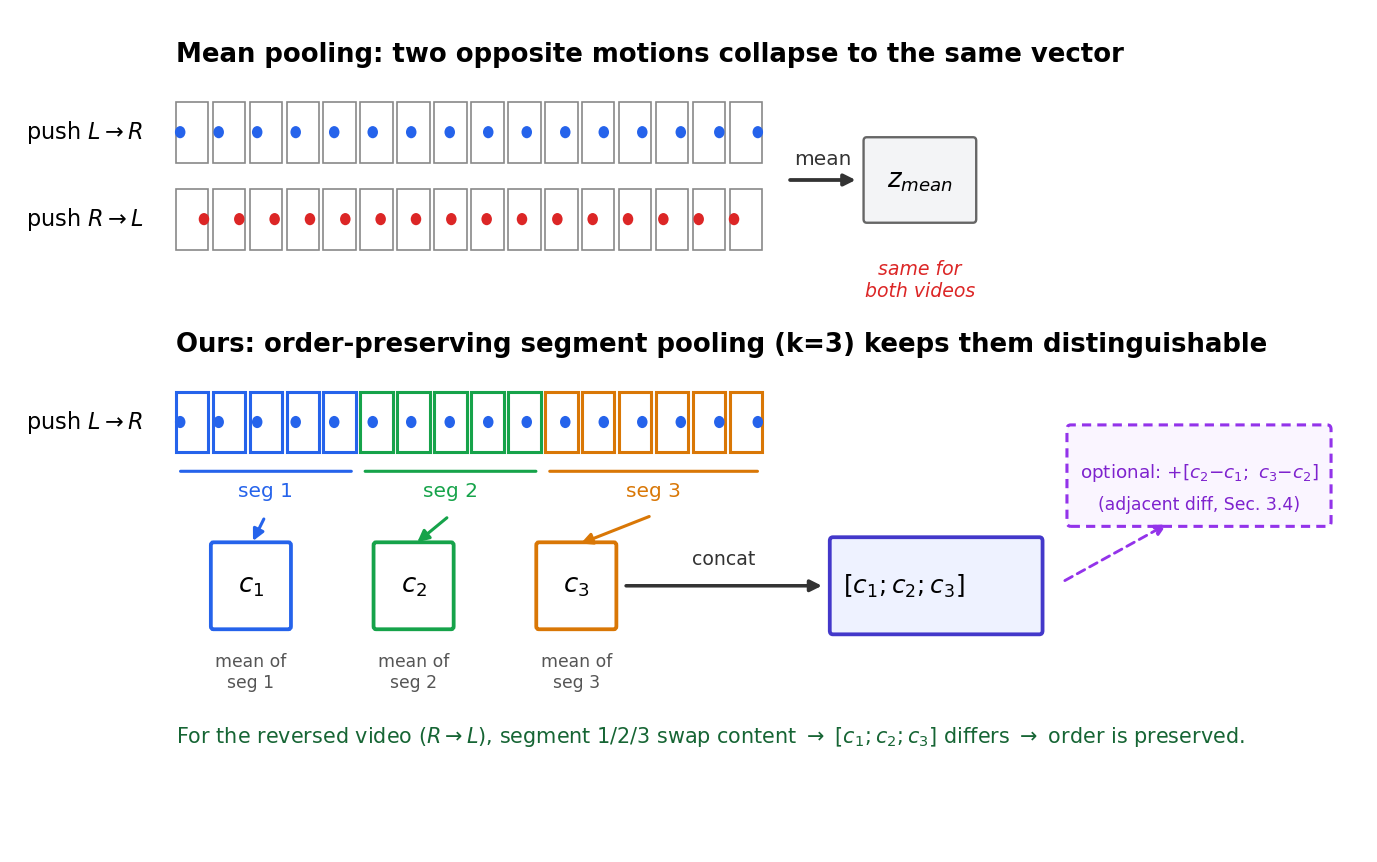
\includegraphics[width=\textwidth]{assets_pooling_diagram.png}
\caption{위: mean pooling은 두 개의 반대 방향 모션(왼쪽에서 오른쪽 vs
오른쪽에서 왼쪽)을 똑같은 벡터 $z_{\mathrm{mean}}$으로 매핑한다.
평균은 프레임 순서에 불변이기 때문이다. 아래: 우리의 순서 보존 segment
pooling($k{=}3$)은 각 시간 구간에 출력 안의 고정된 자리를 부여한다.
$[c_1;c_2;c_3]$를 이어붙이면 어떤 내용이 초반에 있었고 어떤 내용이
후반에 있었는지가 보존되므로, 두 모션은 더 이상 같아지지 않는다.
선택적인 adjacent-difference 항(Section~\ref{sec:method-diff})은 점선으로
분리된 별도 가지로 표시했다. segmentation 자체와는 독립적으로
평가된다는 점을 강조하기 위함이다.}
\label{fig:pooling-diagram}
\end{figure}

\textbf{스코프.} 학습형 temporal encoder(예: ESSENTIAL이 쓰는
transformer)를 붙이면 순서 정보를 복원할 수 있겠지만, 이는
backpropagation을 요구하므로 이 논문의 전제를 포기하는 것이다. 우리는
대신 더 좁고 닫힌 형태의 질문을 던진다: \emph{아무것도 학습시키지 않고
mean pooling이 버리는 시간 정보를 얼마나 되찾을 수 있는가?}

\textbf{제안하는 pooling.} 윈도우 $W \in \mathbb{R}^{T \times D}$
($T{=}16$)를 경계 인덱스
\begin{equation}
b_i = \left\lfloor \frac{iT}{k} \right\rfloor, \quad i = 0,1,\ldots,k
\end{equation}
로 $k$개의 연속된 구간으로 나눈다($T$가 $k$로 나누어떨어지지 않으면 뒤쪽
구간이 남는 프레임을 흡수한다. 예컨대 $T{=}16,\,k{=}3$이면 구간은
$5/5/6$ 프레임이다). 각 구간은 자신의 평균으로 줄어든다:
\begin{equation}
c_i = \frac{1}{b_i - b_{i-1}} \sum_{t=b_{i-1}}^{b_i - 1} W_t \;\in\; \mathbb{R}^D,
\quad i = 1,\ldots,k .
\end{equation}
구간만 쓰는 pooling은 이어붙이기(concatenation)로 순서를 보존한다:
\begin{equation}
\phi_{\mathrm{seg}}(W) = [c_1;\,c_2;\,\ldots;\,c_k] \in \mathbb{R}^{kD}
\;\Longrightarrow\; D'(k) = kD .
\end{equation}
선택적 변형은 인접 구간 간의 차이를 추가로 이어붙이는데, 이는 별개의
메커니즘으로 취급되어 Section~\ref{sec:method-diff}에서 독립적으로 평가된다:
\begin{equation}
\phi_{\mathrm{seg+diff}}(W) = [c_1;\ldots;c_k;\; c_2{-}c_1;\ldots;c_k{-}c_{k-1}]
\in \mathbb{R}^{(2k-1)D}
\;\Longrightarrow\; D'(k) = (2k-1)D ,
\end{equation}
$k$개 구간이면 인접 쌍이 $k{-}1$개 생기기 때문이다. $\phi$의 두 변형
모두 \emph{파라미터 0개, gradient step 0회, 학습 0회}다. 각각은
$(16,512)$ 배열에 대한 고정 함수일 뿐이다. $D{=}512$(CLIP B/32)일 때,
$\mathtt{chunks4}$($k{=}4$, 구간만)는 $D'{=}2048$을,
$\mathtt{chunks3{+}adjdiff}$($k{=}3$, 구간 $+$ diff)는 $D'{=}2560$을
준다. 나머지 조합들과 그 측정된 정확도는 Section~\ref{sec:experiments}에
보고한다.

\textbf{왜 동작하는가.} 두 개의 통제된 관찰이 그 메커니즘을 설명한다.
\emph{첫째}, 성긴 순서만으로도 이득의 대부분을 회복한다: 윈도우를 단 두
구간으로만 나누는 것만으로(``앞 절반은 이랬다'' 대 ``뒤 절반은 이랬다'')
이미 +7.00퍼센트포인트, mean pooling 대비 전체 이득의 78\%를 회복한다.
즉 가장 거친 순서 정보만으로도 대부분의 일을 해낸다는 것이며, 이것이
학습형 pooling이 아니라 닫힌 형태의 pooling 함수를 쓴다는 것의 핵심
직관이다. \emph{둘째}, 순서를 모르는 통계는 도움이 안 된다: 프레임별
표준편차를 추가하는 것(\texttt{mean+std})은 순열 불변이라 출력 차원을
두 배로 늘려도 순서 정보를 전혀 담지 못하며, +1.04\,pp밖에 벌지 못한다.
첫 번째 관찰과 대비하면 이는 차원 자체가 교란 요인이 아님을 배제한다.
이득은 좌표를 추가해서가 아니라 순서를 복원해서 온다.

\textbf{구간 수에 대한 역U자.} $k$를 늘리면 시간 해상도는 좋아지지만
차원 $D'=kD$도 함께 커지고, FeCAM은 클래스당 제한된 샘플 수로
$D' \times D'$ 공분산을 추정해야 한다. 차원 대 샘플 수의 비율이 임계점을
넘으면, 구간을 추가하는 것이 해상도에서 얻는 것보다 추정 오차에서 잃는
게 더 커진다. 그 결과 정확도는 $k$에 대해 역U자를 그리며, 우리 데이터
규모에서는 3~4구간에서 정점을 찍는다(그림~\ref{fig:inverted-u}; 전체
스윕은 Section~\ref{sec:experiments}). 이 시간 해상도 대 추정 가능성의
트레이드오프는 튜닝의 우연이 아니라 이 방법의 내재적 속성이다. 클래스당
사용 가능한 샘플 수가 늘면 최적 $k$도 함께 커질 것으로 예상하지만, 이는
검증하지 않았다.

\begin{figure}[h]
\centering
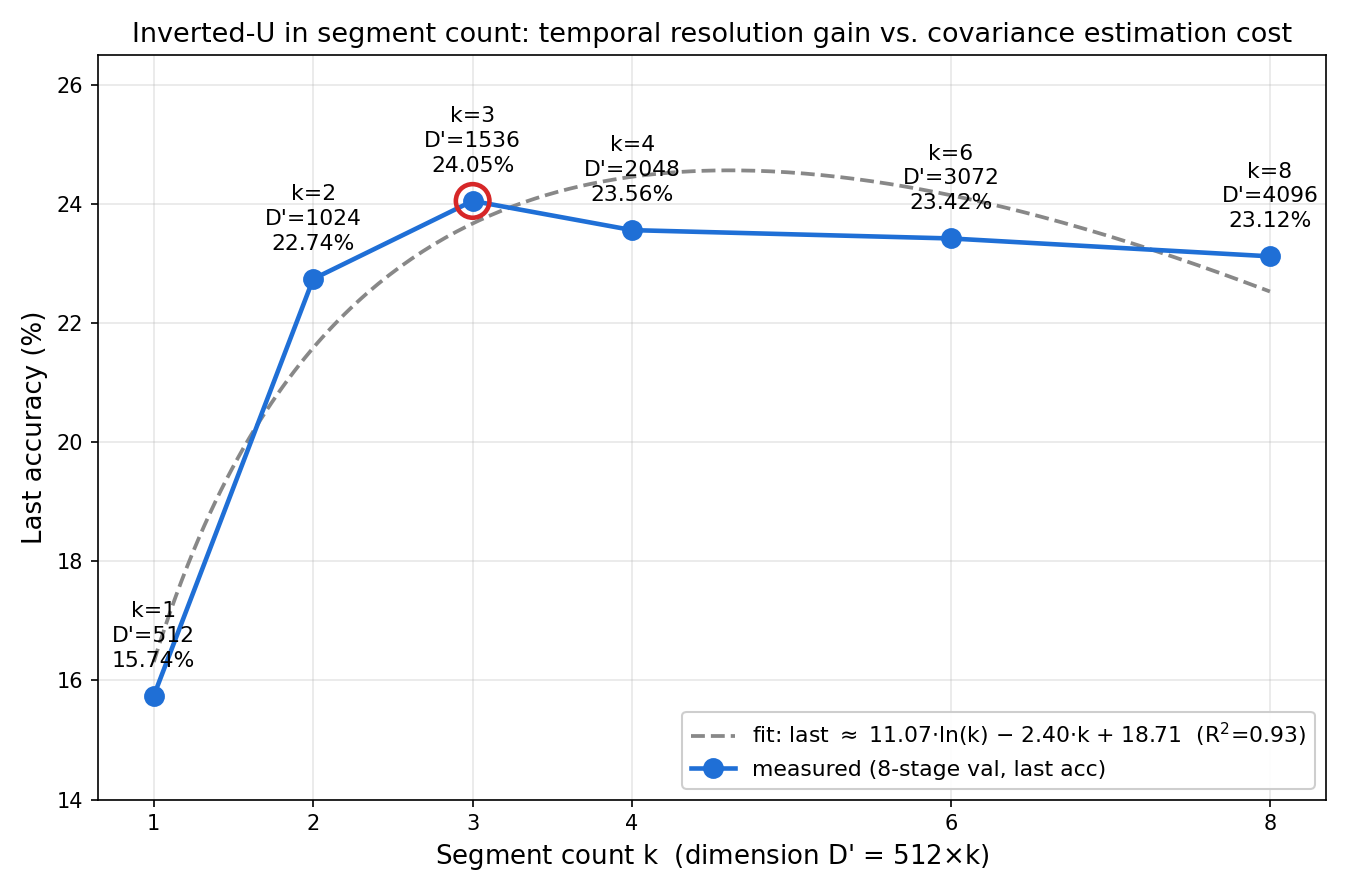
\includegraphics[width=0.75\textwidth]{assets_segment_count_inverted_u.png}
\caption{SSv2(48클래스 프로토콜)에서 구간 수 $k$에 대한 함수로서의
last-session accuracy. 로그-선형 피팅
$\mathrm{Acc}_{\mathrm{last}}(k) \approx 11.07\ln k - 2.40k + 18.71$
($R^2{=}0.93$)은 체감하는 해상도 이득($\ln k$ 항)을 대략 선형인 추정
비용($k$ 항)에 대비시켜 포착한다. $k^*{\approx}4.6$ 부근의 외삽된
최댓값은 그 자체가 실측점이 아니므로 확정된 값이 아니라 예시적인 값으로
읽어야 한다.}
\label{fig:inverted-u}
\end{figure}

\textbf{겹치는 구간은 도움이 안 된다.} 우리는 각 구간을 넓혀 이웃끼리
겹치게 만들면서 총 출력 차원은 $kD$로 고정하는 것도 테스트했다. 이는
convolutional·spectral pooling에서 경계(hard-boundary) 인공물을 고치는
표준적인 처방이다. 이 과제에서는 정확도가 좋아지지 않고 overlap이
커질수록 단조적으로 나빠진다(측정치는 Section~\ref{sec:experiments}). 그
이유는 우연이 아니라 메커니즘적이다: segment pooling이 도움이 되는 것은
각 구간이 출력에서 배타적인 위치를 독점하기 때문이며, 이것이 분류기가
순서를 읽어낼 수 있게 해준다. Overlap은 이웃 구간들이 프레임을 공유하게
만들어, 출력 위치는 여전히 구별되더라도 그 내용이 서로 수렴하게 만든다
(극단적으로는 단순 mean pooling으로 수렴한다). 따라서 윈도우를 넓히는
것은 이 방법이 의존하는 바로 그 속성을 갉아먹는다. 우리는 이를 음성
결과로 보고하며 overlap을 채택하지 않는다.

\subsection{Adjacent and Absolute Difference}
\label{sec:method-diff}

\textbf{서로 다른 두 메커니즘.} Segmentation과 differencing은 메커니즘적으로 서로 다르다: 구간은 윈도우
안의 어떤 콘텐츠가 \emph{어디}에 있는지를 인코딩하고, 인접 구간 간의
차이는 두 위치 사이에서 \emph{무엇이 바뀌었는지}를 인코딩한다. 이 둘을
하나의 관찰로 취급하면 실제 의존관계가 가려진다: differencing이 도움이
되는지는 그것이 프레임 단위에 적용되는지 구간 단위에 적용되는지에 달려
있고, 구간 단위에서는 이미 구간이 몇 개나 있는지에도 달려 있다. 숫자를
보기 전에 그림~\ref{fig:diff-frame-diagram}와~\ref{fig:diff-segment-diagram}
로 두 결과를 먼저 정리한다.

\textbf{프레임 단위.} 외형 정보 없이 연속된 프레임 간의 차이만 쓰면
mean-pooling baseline보다 \emph{더 나쁜} 성능을 낸다. 무언가 움직였다는
걸 아는 것은 무엇이 움직였는지를 모르면 쓸모가 없다. 평균에 프레임 단위
차이를 이어붙이면 상당한 이득을 회복하고, 그 차이의 크기(방향 무관)를
부호 있는 차이 위에 추가로 더하면 더 개선된다. 이 패턴은 구체적인 설계
결론을 뒷받침한다: adjacent/absolute difference는 독립적인 신호가 아니라
외형이 이미 표현되어 있을 때만 도움이 되는 보조 신호다(정량적 값은
Section~\ref{sec:experiments}).

\begin{figure}[ht]
\centering
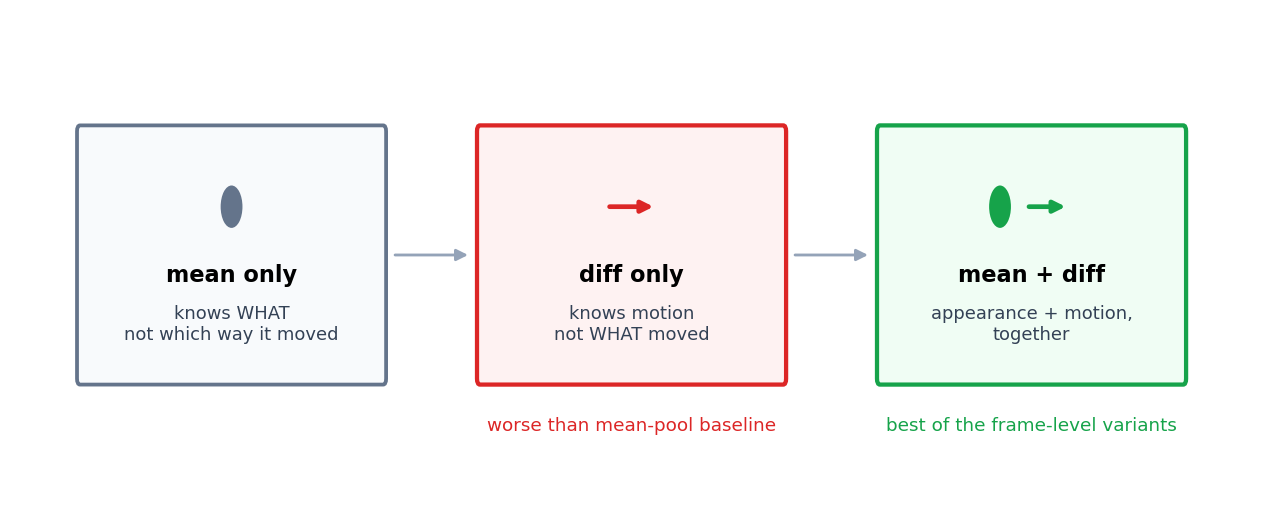
\includegraphics[width=0.85\textwidth]{assets_diff_diagram_frame.png}
\caption{프레임 단위에서는 차이만 쓰면(diff only) 외형 정보를 버려서
mean-pool baseline보다 성능이 낮고, 평균과 차이를 함께 쓰는 것이 프레임
단위 변형 중 가장 좋다.}
\label{fig:diff-frame-diagram}
\end{figure}

\textbf{구간 단위.} 같은 아이디어를 배포 후보인 chunks3와 chunks4에
적용하고 각각에서 차이 항을 켜고 꺼보면 조건부 결과가 나온다: $k{=}3$
에서는 차이 항을 추가하는 것이 일관된 승리다. $k{=}4$에서는 그 효과가
훨씬 약하고, 우리의 두 정확도 지표 중 하나 기준으로는 부호가 뒤집힌다
(Section~\ref{sec:experiments}). 자연스러운 해석은 segmentation과 differencing
이 시간 순서 정보의 출처로서 부분적으로 서로 겹친다는 것이다. 윈도우가
이미 촘촘히 나뉘어 있으면($k{=}4$) 명시적 차이 항이 추가할 수 있는 시간
정보가 그만큼 줄어든다. 이 방향은 독립적인 측정으로도 뒷받침된다.
$k{=}3$/$k{=}4$ 직접 비교와는 별도로 실행한 held-out 선택 스윕이 같은
결론에 도달하며, 이는 단일 실험의 우연이 아니라는 근거가 된다.

\begin{figure}[ht]
\centering
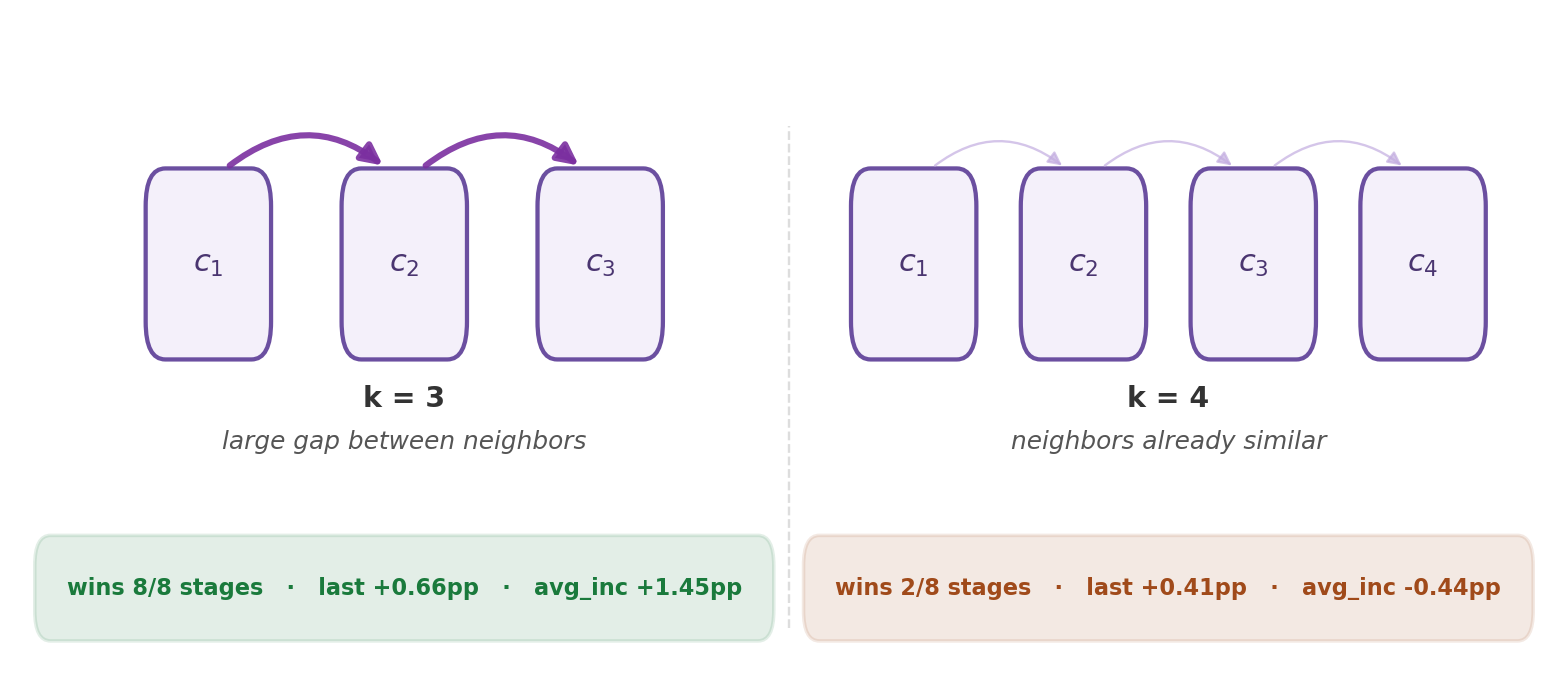
\includegraphics[width=\textwidth]{assets_diff_diagram_segment.png}
\caption{구간 단위에서는 같은 인접 차분 연산 ($c_i{-}c_{i-1}$)이 $k$
값에 따라 정반대의 가치를 갖는다: $k{=}3$처럼 구간이 성기면 이웃한 구간
평균끼리 차이가 크고 diff 항이 모든 평가 스테이지에서 이긴다. $k{=}4$처럼
구간이 촘촘하면 이웃한 구간 평균이 이미 비슷해서 diff 항이 segmentation
자체와 상당 부분 중복되고, 그 이득도 일관되지 않게 된다(화살표 굵기는
이 격차가 줄어든다는 것을 비유적으로 보여줄 뿐, 정확한 비례는 아니다).}
\label{fig:diff-segment-diagram}
\end{figure}


% =====================================================================
\section{Experiments}
\label{sec:experiments}
% =====================================================================

\subsection{Configuration}

\textbf{데이터셋.} UCF101(Soomro et al., arXiv:1212.0402)은 공식
split~1 기준 101개 행동 클래스와 13{,}320개 클립을 제공한다. 우리는
TCD(Park et al., ICCV'21) 프로토콜을 따른다: 51개 base 클래스를
오프라인으로 학습하고, 나머지 50개 클래스를 incremental하게 등록한다.
표~\ref{tab:ucf101-spec}는 원 논문과 대조해 검증한 정확한 데이터셋
스펙이다.

\begin{table}[h]
\centering
\caption{UCF101 스펙(Soomro et al., arXiv:1212.0402).}
\label{tab:ucf101-spec}
\small
\begin{tabular}{@{}L{3.5cm}L{6cm}@{}}
\toprule
항목 & 값 \\
\midrule
클래스 수 & 101 \\
총 클립 수 & 13{,}320 \\
클래스당 그룹 수 & 25 \\
그룹당 클립 수 & 4--7 \\
총 재생시간 & 1{,}600분 \\
클립 길이 범위 & 1.06\,s -- 71.04\,s \\
프레임레이트 & 25\,fps \\
해상도 & $320\times240$ \\
출처 & YouTube (2012) \\
\bottomrule
\end{tabular}
\end{table}

Something-Something V2(Goyal et al., ICCV'17; V2 재배포는 Qualcomm 공식
배포 기준)는 외형보다는 상당 부분 모션으로 정의되는 174개 행동 클래스를
제공한다. 우리는 두 규모를 병행 사용한다: (1) 대부분의 ablation·head
비교에 쓰는 큐레이션된 48클래스 부분집합(클래스당 최대 100개 학습 샘플,
8단계 $\times$ 6클래스 커리큘럼), (2) TCD의 리터럴 프로토콜(84 base $+$
$10{\times}9$ 또는 $5{\times}18$ incremental 세션)을 재현하기 위한
174클래스 전체(클래스당 학습 100개/검증 50개 상한). 표
\ref{tab:ssv2-spec}가 전체 스펙이다.

\begin{table}[h]
\centering
\caption{SSv2 스펙.}
\label{tab:ssv2-spec}
\small
\begin{tabular}{@{}L{3.5cm}L{9cm}@{}}
\toprule
항목 & 값 \\
\midrule
클래스 수 & 174 \\
총 비디오 수 & 220{,}847 \\
train / val / test & 168{,}913 / 24{,}777 / 27{,}157(라벨 없음) \\
크라우드 작업자 & 5{,}400명 이상 \\
프레임레이트 & 12\,fps(실측) \\
코덱 / 컨테이너 & VP9, WebM \\
해상도(높이) & 240\,px \\
클립 길이 & 약 2--6\,s(문헌); 실측 샘플: 3.08\,s(37프레임), 4.67\,s(56프레임) \\
총 다운로드 용량 & 19.4\,GB \\
\bottomrule
\end{tabular}
\end{table}

\textbf{특징 추출.} 두 데이터셋 모두 클립당 16프레임을 균등 샘플링하고
(\texttt{av}로 디코딩), frozen CLIP ViT-B/32
(\texttt{openai/clip-vit-base-patch32}, 512-d)로 독립적으로 인코딩해
클립당 $(16, D)$ 원시 특징을 만든다. 두 데이터셋 모두에서 backbone은
고정되며, 어떤 단계에서도 gradient가 흐르지 않는다. Pooling은 이 원시
특징에 평가 시점에 적용되므로, pooling 변형은 고정된 입력 위에서 $\phi$를
고르는 문제이지 특징을 다시 뽑는 것이 아니다. 표에 달리 명시하지 않는 한
주요 결과는 \texttt{chunks3+adjdiff}를 쓰며, mean pooling은 비교 대상인
baseline으로만 등장한다.

\textbf{클래스 순서와 분할.} 결과가 클래스 순서의 우연에 좌우되지
않도록, base/incremental 분할은 고정된 랜덤 시드 순열로 생성하며, 여러
시드에 걸쳐 보고하는 결과는 최소 3개 이상의 클래스 순서에 대해 평균낸다.

\textbf{하이퍼파라미터.} 표~\ref{tab:hyperparams}는 아래 실험에서 쓰인
모든 하이퍼파라미터를 나열한다.

\begin{table}[h]
\centering
\caption{하이퍼파라미터.}
\label{tab:hyperparams}
\small
\renewcommand{\arraystretch}{1.15}
\begin{tabular}{@{}L{4.3cm}L{9.5cm}@{}}
\toprule
구성요소 & 설정값 \\
\midrule
프레임 수(클립당) & 16(균등 샘플링) \\
Pooling 차원 배율 & mean $1\times$(512-d) / chunks4 $4\times$(2048-d) / chunks3+adjdiff $5\times$(2560-d) \\
FeCAM shrinkage & 대각 $\gamma_1{=}1.0$, 비대각 $\gamma_2{=}1.0$(many-shot CIL 설정, Goswami et al.\ 2023) \\
FeCAM few-shot correction & 배포 설정에서 활성화; 균형 표본에서는 no-op \\
SLDA shrinkage & 등방(isotropic) $\lambda{=}0.01$(대각에만 적용) \\
SSv2 48-class curriculum & 8단계 $\times$ 6클래스 \\
SSv2 174-class(TCD) 구조 & 84-class base $+$ 90-class incremental($10{\times}9$ 또는 $5{\times}18$ 세션) \\
UCF101(TCD) 구조 & 51-class base $+$ 50-class incremental(baseline은 5-shot/class exemplar) \\
실시간 목표 & 10\,fps($=$100\,ms/frame), CPU, batch$=$1(스트리밍) \\
타이밍 측정 하드웨어 & Apple M4, 10코어(성능 4 $+$ 효율 6), 16\,GB RAM \\
\bottomrule
\end{tabular}
\end{table}

\textbf{평가 지표.} 우리는 두 개의 정확도 지표와 두 개의 효율성 지표를
보고하며, 표~\ref{tab:metrics}에 정의돼 있다. Average incremental
accuracy($\mathrm{Acc}_{\mathrm{avg}}$)는 iCaRL 이후 CIL 문헌의 표준
헤드라인 지표다. Last-session accuracy($\mathrm{Acc}_{\mathrm{last}}$)는
더 어렵고 순서에 불변인 수치로, 클래스 수가 다른 벤치마크를 비교할
때는 반드시 이걸 써야 한다. $\mathrm{Acc}_{\mathrm{avg}}$는 클래스가 더
적은 초반 세션 때문에 체계적으로 부풀려지기 때문이다. 별도로 명시하지
않는 한 보고된 모든 정확도는 완전한 class-incremental 평가(지금까지 본
모든 클래스에 대한 argmax, 테스트 시 태스크/세션 식별자 없음)를 쓴다.

\begin{table}[h]
\centering
\caption{지표 정의.}
\label{tab:metrics}
\small
\begin{tabular}{@{}lL{6.3cm}L{5.7cm}@{}}
\toprule
지표 & 정의 & 용도 \\
\midrule
$\mathrm{Acc}_s$ & 세션 $s$까지 본 모든 클래스에 대한 val accuracy & 증분 곡선의 한 점 \\
$\mathrm{Acc}_{\mathrm{avg}}$ & $\frac{1}{S}\sum_{s=1}^{S}\mathrm{Acc}_s$ & 헤드라인 지표(iCaRL 관례) \\
$\mathrm{Acc}_{\mathrm{last}}$ & 마지막 세션의 accuracy & 가장 어렵고 순서 불변; 벤치마크 간 비교에 필요 \\
\midrule
FPS & $1000 / (\text{encode}_{\text{1frame}} + \text{pool} + \text{head\_scores})$, ms & 스트리밍 처리율(ring buffer, CPU, batch$=$1) \\
Fit time & 한 세션 분량으로 head를 갱신하는 wall-clock & 등록(enrollment) 비용 \\
\bottomrule
\end{tabular}
\end{table}

\subsection{Results and Discussion}

\textbf{닫힌 형태 대 backprop의 비용 격차.} 이 설계의 동기가 된
등록(enrollment) 비용 주장(Section~\ref{sec:intro})은 가정이 아니라 직접
측정한 것이다. 측정은 Apple M4 CPU(10코어: 성능 4개 $+$ 효율 6개,
16\,GB RAM)에서 이루어졌다. 우리 48클래스 SSv2 프로토콜(8 stage,
stage당 15 epoch)에서 FeCAM head를 fit하는 데는 wall-clock 42.4\,ms가
걸리는 반면, 같은 데이터로 작은 GRU baseline(hidden 256, Adam, 학습률
$10^{-4}$, binary cross-entropy loss)을 backpropagation으로
fine-tune하는 데는 270.0\,s가 걸린다: 격차는
$6{,}400\times$다. 하드웨어에 무관한 회계로도 같은 결론이 나온다:
FeCAM의 학습 FLOPs는 2.85\,G인 반면 GRU baseline은 4.64\,T로,
$1{,}628\times$ 더 적다.

\textbf{UCF101(TCD 프로토콜)에서 선행 연구와의 비교.} 우리는 프로토콜
일치를 가정하지 않고 직접 검증했다: 우리 클래스 순서는 TCD의 공개
저장소와 101개 클래스 전부에서 비트 단위로 일치한다. 표
\ref{tab:ucf101-compare}는 우리 방법을 이 프로토콜에서 자체 보고된
다섯 방법과 나란히 놓는다. 우리는 exemplar 0개, gradient step 0회를
쓰면서도 TCD보다 15.1\,pp, FrameMaker보다 11.9\,pp, STSP보다 8.9\,pp,
ST-Prompt보다 5.2\,pp 앞서고 ESSENTIAL 다음으로 2위를 차지한다.

\begin{table}[h]
\centering
\caption{UCF101, TCD 프로토콜, 세 가지 증분 단위에서의 average
incremental accuracy(각 논문 자체 보고치). 우리 행은 SSv2에서 선택한
\texttt{chunks3+adjdiff} pooling(Section~\ref{sec:method-pooling})을
그대로 적용한 것이다. 동일한 프로토콜에서 mean-pool baseline은
88.84/88.86/88.84이므로, 우리 격차 중 $+1.16$\,pp는 pooling 자체에서
온다. \texttt{chunks4+adjdiff}가 여기서는 근소하게 더 높지만(90.23),
바꿔 넣지 않았다: pooling 선택은 UCF101을 보기 전에 SSv2에서 이미
고정했고, 여기서 바꾸면 test set을 보고 고르는 셈이 되기 때문이다.
TCD와 FrameMaker(Pei 등,
NeurIPS'22, arXiv:2211.00833)는 둘 다 TSM backbone을 학습 내내
fine-tune하며, 각각 클래스당 exemplar 5개와 미공개 개수를 재생한다.
STSP는 exemplar-free이며 표~\ref{tab:tcd-lineage}와 동일한 방법을
SSv2 대신 UCF101에서 평가한 것이다. ST-Prompt(Pei 등, ICCV'23)는 CLIP은
고정한 채 space-time prompt를 backpropagation으로 학습시킨다.
ESSENTIAL은 CLIP은 고정하지만 temporal encoder와 classifier를
backpropagation(24$\times$RTX~3090)으로 학습시킨다. 우리는 exemplar
0개, 어떤 시점에서도 gradient step 0회인 frozen CLIP을 쓴다. 여기서 우리
$\mathrm{Acc}_{\mathrm{avg}}$는 마지막 세션을 포함한 전체 $S$개 세션에
대한 평균이다(표~\ref{tab:metrics}). TCD/FrameMaker/ST-Prompt 자체
관례(CSTA 논문 대조로 확인)는 대신 마지막을 제외한 첫 $S{-}1$개 세션만
평균내는데, 그 방식대로 우리 값을 다시 계산하면 89.12/89.00/88.90이
나온다. 순위에는 영향 없는 0.06--0.28\,pp 차이다.}
\label{tab:ucf101-compare}
\small
\begin{tabular}{@{}lccc@{}}
\toprule
방법 & $10\times5$ & $5\times10$ & $2\times25$ \\
\midrule
TCD (ICCV'21) & 74.89 & 73.43 & 72.19 \\
FrameMaker (NeurIPS'22) & 78.13 & 76.38 & 75.77 \\
STSP (ECCV'24) & 81.15 & 82.84 & 79.25 \\
ST-Prompt (ICCV'23) & 84.80 & 85.50 & 85.70 \\
\textbf{Ours (frozen CLIP + FeCAM + \texttt{chunks3+adjdiff})} & \textbf{90.00} & \textbf{89.99} & \textbf{89.97} \\
ESSENTIAL (ICCV'25) & 95.1 & 93.9 & 93.3 \\
\bottomrule
\end{tabular}
\end{table}

\textbf{증분 단위에 대한 불변성.} 표~\ref{tab:invariance}는 우연이
아니라 구조적 속성을 보여준다. 증분을 점점 더 작은 그룹으로 쪼갤수록
다른 모든 방법의 정확도는 움직인다. 대체로 하락하지만(TCD
$-2.70$\,pp, FrameMaker $-2.36$\,pp, ESSENTIAL $-1.80$\,pp), 어떤 경우는
비단조적이고(STSP는 중간 단위에서 한 번 올랐다가 떨어져 순변화
$-1.90$\,pp), 어떤 경우는 오히려 오른다(ST-Prompt, $+0.90$\,pp). 우리
방법은 $-0.03$\,pp 움직이는데, 이들 중 어느 것보다도 한 자릿수 작다.
남은 0.03은 모델이 흔들린 것이 아니라 지표의 산물이다:
$\mathrm{Acc}_{\mathrm{avg}}$는 스케줄이 정의하는 평가 지점들을 평균내는데,
세 스케줄이 정의하는 지점 수가 각각 6개, 11개, 26개로 다르기 때문이다.
구성상 불변인 양은 101개 클래스를 모두 등록한 뒤의 정확도
$\mathrm{Acc}_{\mathrm{last}}$이며, 이 값은 세 스케줄 모두에서 88.61로
비트 단위까지 동일하다. 둘 다 닫힌 형태 갱신 규칙에서 나온다: running
mean과 공분산은 기저 샘플들이 어떤 순서·묶음으로 도착하든 같은 통계값으로
수렴하며, 이는 이 표의 어떤 gradient 학습 방법도 갖지 못한 보장이다. 실용적 함의는 정확도
우위가 아니라 배포 신뢰성이다: 새로 도착하는 클래스의 수와 시점을 미리
알 수 없는 환경에서, 이 속성은 불리한 등록 스케줄로도 성능이 어느
방향으로든 흔들릴 수 없음을 보장한다.

\begin{table}[h]
\centering
\caption{UCF101에서 가장 성긴 증분 단위에서 가장 잘게 쪼갠 증분 단위로
갈 때의 정확도 변화(표~\ref{tab:ucf101-compare}와 동일한 방법들).
$^\dagger$STSP는 세 증분 단위에서 비단조적이다(81.15 $\to$ 82.84
$\to$ 79.25). 여기 표시된 값은 양 끝점만 쓴 것이다.}
\label{tab:invariance}
\small
\begin{tabular}{@{}lc@{}}
\toprule
방법 & $10\times5 \to 2\times25$ \\
\midrule
TCD & $74.89 \to 72.19$ ($-2.70$) \\
FrameMaker & $78.13 \to 75.77$ ($-2.36$) \\
STSP$^\dagger$ & $81.15 \to 79.25$ ($-1.90$) \\
ST-Prompt & $84.80 \to 85.70$ ($+0.90$) \\
ESSENTIAL & $95.1 \to 93.3$ ($-1.80$) \\
\textbf{Ours} & $90.00 \to 89.97$ (\textbf{$-0.03$}) \\
\bottomrule
\end{tabular}
\end{table}

\textbf{Ablation: 구간 수.} 그림~\ref{fig:inverted-u}는 정확도가 3~4
구간에서 정점을 찍고 그 이후로는 하락함을 보여주며, 더 잘게 나눌수록
단순히 더 좋아지는 게 아님을 확인해준다. Section~\ref{sec:method-pooling}의
시간 해상도/공분산 추정 가능성 트레이드오프가 실재하고 측정 가능하다.

\textbf{Ablation: adjacent/absolute difference.} 표
\ref{tab:diff-frame}는 segmentation이 도입되기 전 프레임 단위에서의
differencing 효과를 분리한다: differencing만으로는(외형 없이)
mean-pool baseline보다 성능이 낮고, 부호 있는 차이를 추가한 뒤 그
크기까지 추가하면 꾸준히 개선된다.

\begin{table}[h]
\centering
\caption{프레임 단위 diff ablation(mean 512-d baseline). O는 포함된
컴포넌트를 표시.}
\label{tab:diff-frame}
\small
\begin{tabular}{@{}cccccc@{}}
\toprule
mean & std & diff & $|$diff$|$ & 차원 & $\mathrm{Acc}_{\mathrm{avg}}$ / $\mathrm{Acc}_{\mathrm{last}}$ \\
\midrule
O & & & & 512 & 24.19 / 15.74 \\
O & O & & & 1024 & 24.69 / 16.78 \\
 & & O & & 512 & 22.65 / 13.12 \\
O & & O & & 1024 & 30.50 / 20.69 \\
O & & O & O & 1536 & 30.82 / 21.50 \\
\bottomrule
\end{tabular}
\end{table}

표~\ref{tab:diff-segment}는 같은 질문을 두 배포 후보 pooling에 대해
구간 단위로 분리한다. $k{=}3$에서는 차이 항을 추가하는 것이 8개 평가
스테이지 중 8개 전부에서 이긴다. $k{=}4$에서는 6번, 8번 스테이지에서만
이기고 나머지 여섯 곳에서는 진다($-1.83$~$-0.05$\,pp). 이것이
$\mathrm{Acc}_{\mathrm{last}}$ 기준으로는 (아슬아슬하게) 양수를
유지하면서도 $\mathrm{Acc}_{\mathrm{avg}}$ 기준으로는 부호가 뒤집히는
이유다. \texttt{chunks4+adjdiff}는 네 조합 중 가장 비싸면서(차원 3584,
fit 10.4\,s) 도움이 될지 가장 불확실한 조합이기도 해서, 배포에서 제외할
근거가 된다.

\begin{table}[h]
\centering
\caption{배포 후보들에 대한 구간 단위 diff ablation.}
\label{tab:diff-segment}
\small
\begin{tabular}{@{}lccccc@{}}
\toprule
& diff 없음(차원) & diff 추가(차원) & $\Delta\,\mathrm{Acc}_{\mathrm{last}}$ & $\Delta\,\mathrm{Acc}_{\mathrm{avg}}$ & 이긴 스테이지(8개 중) \\
\midrule
$k{=}3$ & 24.05 (1536) & \textbf{24.71} (2560) & \textbf{+0.66} & +1.45 & \textbf{S1--S8 (8/8)} \\
$k{=}4$ & 23.56 (2048) & 23.97 (3584) & $+0.41$ & \textbf{$-0.44$} & S6, S8만(2/8) \\
\bottomrule
\end{tabular}
\end{table}

\textbf{표준 174클래스 split으로의 확장.} 위 ablation들은 우리 48클래스
커리큘럼을 쓴다. 표~\ref{tab:tcd-lineage}는 SSv2의 실제 174클래스 TCD
split에서 선행 연구를 정리했지만 우리 방법은 거기 없었다.
표~\ref{tab:ssv2-174}가 그 빈틈을 메운다. FeCAM head를 고정하고 같은
pooling 변형들을 스윕한다. 이 스케일에서도 order-preserving pooling은
mean pooling을 큰 폭으로 이기며, \texttt{chunks3+adjdiff}가 테스트한
모든 변형 중 다시 1등이다. mean pooling 대비
$+6.77$\,pp $\mathrm{Acc}_{\mathrm{last}}$, $+6.74$\,pp
$\mathrm{Acc}_{\mathrm{avg}}$. 한 가지 순위는 반복되지 않는다: diff
없이는 \texttt{chunks4}가 여기서 \texttt{chunks3}를 근소하게
앞선다($0.24$\,pp $\mathrm{Acc}_{\mathrm{last}}$), 48클래스에서의 순서
(\texttt{chunks3}가 $0.49$\,pp 앞섬, 표~\ref{tab:diff-segment}의
diff-없음 열)와는 반대다. 두 격차 모두 이번 실험의 seed 간 노이즈
범위 안이다($\mathrm{Acc}_{\mathrm{avg}}$ 기준 $\pm0.18$--$0.20$\,pp).
diff 항을 더하면 두 스케일 모두에서 순위가 명확해진다.
$\mathrm{Acc}_{\mathrm{last}}$는 여기서도 정확히 불변이다: 세 seed
전부와 $10{\times}9$/$5{\times}18$ 두 스케줄 사이에서 표시된 자릿수까지
동일하다. UCF101에서 표~\ref{tab:invariance}가 확립한 것과 같은 구조적
속성이 이제 두 번째 데이터셋에서, 클래스 수 $3.6$배 규모로 확인된
것이다. 절대 정확도는 표~\ref{tab:tcd-lineage}의 backprop 학습 방법들보다
여전히 많이 낮다(여기서는 18.50, 그 표에서 가장 강한 항목인 STSP의
70.87과 비교하면). Section~\ref{sec:related}가 이미 그 이유를 설명한다:
그 방법들은 backbone을 SSv2 모션에 적응시키지만 우리는 한 번도 그렇게
하지 않기 때문이다. 이 trade-off는 부수적인 게 아니라 명시적인 설계다:
이 논문은 mean pooling이 버리는 순서 신호를 복원할 뿐, SSv2 모션으로
아예 학습시키는 데서 오는 더 큰 격차를 메우려는 것이 아니다.

\begin{table}[h]
\centering
\caption{SSv2의 표준 174클래스 TCD split(84 base $+$ 90 incremental
클래스)에서의 order-preserving pooling, FeCAM head, 3개 seed에 대한
평균 $\pm$ 표준편차. TCD 자체의 84클래스 base 목록은 공개되어 있지
않으므로, 여기서는 문헌의 실제 split을 재현하는 대신 seed마다 무작위
분할을 사용한다(구조와 규모만 재현하며 정확한 클래스 배정은 아니다).
$\mathrm{Acc}_{\mathrm{last}}$는 seed 사이에서도, $10{\times}9$/
$5{\times}18$ 스케줄 사이에서도 표시된 자릿수까지 변하지 않는다.}
\label{tab:ssv2-174}
\small
\begin{tabular}{@{}lcccc@{}}
\toprule
Pooling & $D$ & $\mathrm{Acc}_{\mathrm{last}}$ & $\mathrm{Acc}_{\mathrm{avg}}$ ($10{\times}9$) & $\mathrm{Acc}_{\mathrm{avg}}$ ($5{\times}18$) \\
\midrule
mean & 512 & 11.74 & 14.42 $\pm$ 0.19 & 14.39 $\pm$ 0.20 \\
chunks3 & 1536 & 17.55 & 20.46 $\pm$ 0.19 & 20.42 $\pm$ 0.19 \\
chunks4 & 2048 & 17.79 & 20.81 $\pm$ 0.19 & 20.76 $\pm$ 0.18 \\
\textbf{chunks3+adjdiff} & 2560 & \textbf{18.50} & \textbf{21.17 $\pm$ 0.14} & \textbf{21.12 $\pm$ 0.16} \\
chunks4+adjdiff & 3584 & 18.15 & 20.98 $\pm$ 0.29 & 20.95 $\pm$ 0.28 \\
\bottomrule
\end{tabular}
\end{table}

\textbf{Ablation: head 선택.} 표~\ref{tab:head-ladder}는
Section~\ref{sec:method-fecam}의 NCM $\to$ SLDA $\to$ FeCAM 사다리를 실증적
으로 확인해준다: head가 공분산 구조를 얼마나 쓰는지에 따라 정확도가
단조적으로 오르며, 대가는 더 높아진(그래도 1초 미만인) fit 시간이다.

\begin{table}[h]
\centering
\caption{SSv2(48클래스 프로토콜)에서의 head 비교.}
\label{tab:head-ladder}
\small
\begin{tabular}{@{}lccc@{}}
\toprule
Head & $\mathrm{Acc}_{\mathrm{avg}}$ & $\mathrm{Acc}_{\mathrm{last}}$ & Fit time (s) \\
\midrule
NCM & 20.89 & 12.38 & 0.08 \\
SLDA & 22.77 & 14.14 & 0.13 \\
\textbf{FeCAM} & \textbf{24.19} & \textbf{15.74} & 0.40 \\
\bottomrule
\end{tabular}
\end{table}

\textbf{최적의 배포 가능한 조합 찾기.} 마지막으로 그림
\ref{fig:combo-sweep}는 CLIP B/32 위에서 아홉 개의 pooling$\times$head
조합 전부를 하나의 정확도-대-처리율 평면에 놓는다. 아홉 조합 모두
10\,fps 실시간 예산을 큰 폭으로(39.4--41.6\,fps) 넘어서므로, 이 스코프
안에서는 처리율이 선택을 제약하지 않는다. 결정은 정확도만으로 귀결되고,
FeCAM은 테스트한 모든 pooling 변형에서 NCM과 SLDA를 압도한다.

\begin{figure}[h]
\centering
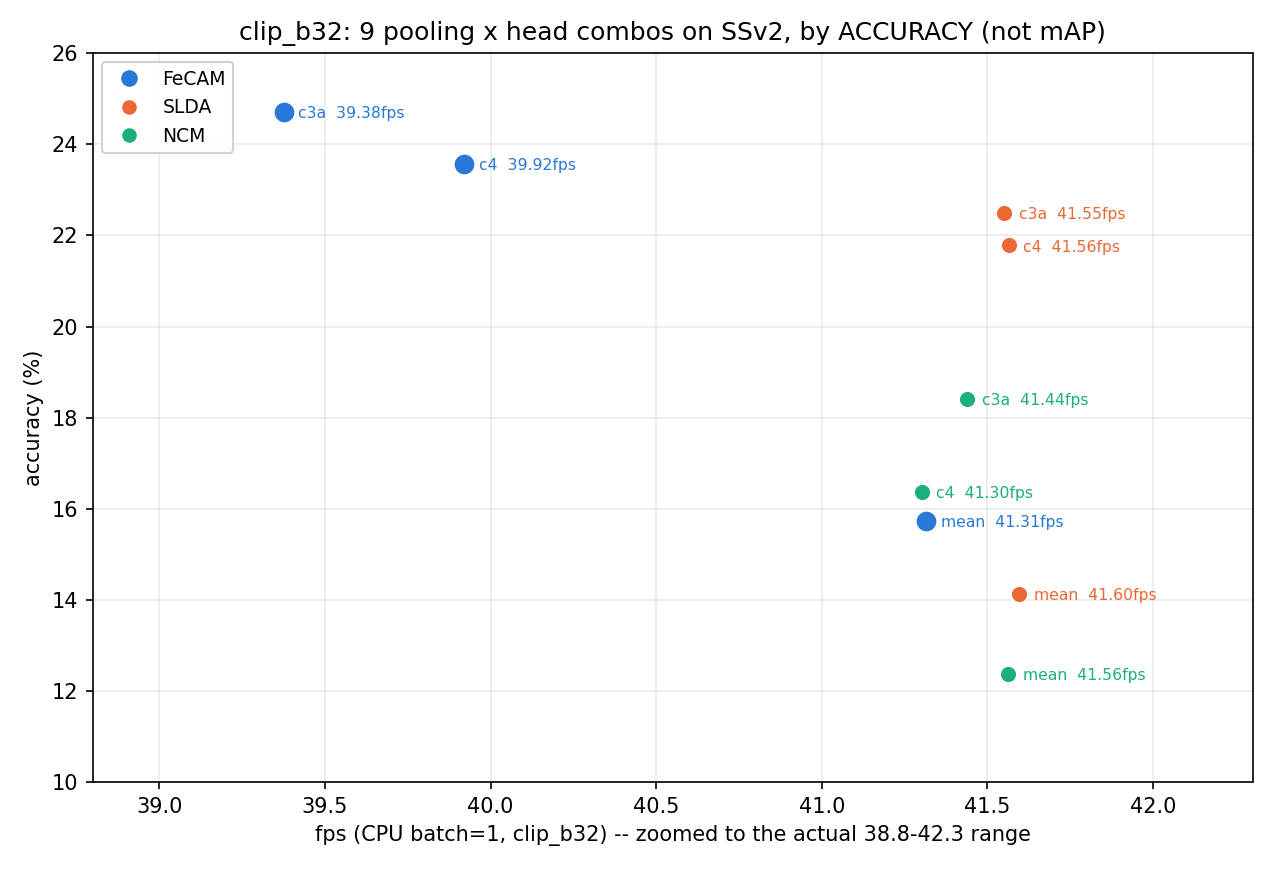
\includegraphics[width=0.8\textwidth]{assets_ap_fps_sweep_accuracy.png}
\caption{SSv2(CLIP B/32, CPU, batch$=$1)에서 아홉 개
pooling$\times$head 조합의 정확도 대 처리율. 아홉 조합 전부 10\,fps
예산 안에 여유 있게 들어온다. FeCAM이 모든 pooling 설정에서 앞선다.}
\label{fig:combo-sweep}
\end{figure}


% =====================================================================
\section{Conclusion}
\label{sec:conclusion}
% =====================================================================

\textbf{요약.} 이 논문은 비디오 class-incremental learning을 GPU 없이,
exemplar replay 없이, 배포 이후 gradient step 단 한 번도 없이 동작하게
만들 수 있는지를 물었다. 이미 image CIL에서 통하는 레시피, 즉 frozen
backbone과 닫힌 형태(closed-form) 공분산 head에서 출발해, 그 레시피가
비디오에서 빠뜨리고 있는 단 하나의 요소를 짚었다: 프레임의 순서를
평균으로 지우는 대신 보존하는 방법이다. Order-preserving temporal
pooling은 각 윈도우를 $k$개의 연속된 구간으로 나누고 그 평균들을
이어붙여, early-then-late와 late-then-early가 같은 좌표가 아니라 서로
다른 좌표를 차지하게 함으로써 이 빈틈을 메운다. Pooling 함수와 FeCAM
head는 둘 다 frozen-backbone 파이프라인에 학습 파라미터 0개, gradient
step 0회만을 더한다.

\textbf{Ablation이 보여주는 것.} 이득은 점진적이라기보다는 초반에
집중되어 있고 메커니즘적이다. 윈도우를 단 두 구간으로만 나누어도 이미
mean pooling 대비 전체 개선의 78\%를 회복하며, 정확도는 구간 수에 대해
단조 상승이 아니라 우리 데이터 규모에서 $k{=}3$--$4$에서 정점을 찍는
역U자를 그린다. 이는 ``구간이 많을수록 좋다''는 설명을 배제한다.
이웃끼리 겹치도록 구간을 넓히는 것, 즉 다른 분야에서 경계
인공물(boundary artifact)에 쓰이는 표준적인 처방은, 이 과제에서는
오히려 정확도를 단조적으로 떨어뜨린다: overlap은 정확히 이 방법이
의존하는 그 속성을 갉아먹기 때문이다. Adjacent-frame differencing은
외형이 이미 표현되어 있을 때는 도움이 되지만 그 자체로는 오히려 해가
되며, 구간 단위에서는 그 가치가 조건부다: $k{=}3$에서는 일관된
승리(8개 스테이지 중 8개)이지만 $k{=}4$에서는 미미하고 부호가 뒤집히는
수준(8개 중 2개)이다. 이는 segmentation과 differencing이 공짜로 쌓이는
게 아니라 시간 순서 정보의 출처로서 부분적으로 서로 겹친다는 근거다.
같은 순위, 즉 \texttt{chunks3+adjdiff}가 테스트한 다른 모든 pooling을
앞서는 순위는 SSv2의 표준 174클래스 split, 클래스 수 $3.6$배
규모에서도 재현되며(표~\ref{tab:ssv2-174}), UCF101에서
표~\ref{tab:invariance}가 확립한 것과 같은 정확한 last-session
불변성도 함께 재현된다.

\textbf{선행 연구 대비 위치.} TCD 프로토콜 기준 UCF101에서 이 방법은
ESSENTIAL에만 뒤지는 2위이며, TCD·FrameMaker·STSP·ST-Prompt보다
앞선다. 그 표의 다른 모든 방법이 exemplar나 gradient step 중 최소
하나는 쓰는 반면 이 방법은 둘 다 0이다. 그 표의 어느 방법도 갖지 못한
속성도 있다: 증분 세션을 얼마나 거칠게 또는 잘게 묶든 정확도가
불변이다. 마지막 세션 정확도는 $10\times5$, $5\times10$, $2\times25$
세 스케줄에서 비트 단위까지 동일하고, average incremental accuracy는
$-0.03$\,pp 움직인다(TCD는 $-2.70$\,pp, ESSENTIAL은 $-1.80$\,pp). 이
불변성은 튜닝의 결과가 아니라 닫힌 형태 갱신이 도착 순서와 무관하다는
데서 직접 따라 나오는 귀결이며, 표에서의 순위 자체보다 운영상 더
중요하다: 배포된 시스템은 클래스가 어떤 순서로 도착할지 항상 통제할 수
없는데, 이 속성은 어떤 등록 스케줄로도 성능이 더 나빠지지 않음을
보장한다. 테스트한 아홉 개의 pooling$\times$head 조합 전부가 10\,fps
실시간 예산을 여유 있게(CPU에서 39.4--41.6\,fps) 넘어서므로, 이 순위는
처리율을 희생해서 얻은 것이 아니다.

\textbf{한계.} 두 가지 스코프 선택은 분명히 밝혀야 한다. 첫째,
표~\ref{tab:ssv2-174}는 SSv2의 표준 174클래스 split에 대한 우리 자신의
수치를 보고하지만, TCD 자체의 84클래스 base 목록은 공개되어 있지
않으므로 그 base/incremental 분할은 문헌의 실제 split을 재현한 것이
아니라 seed마다 무작위로 정한 것이다. 이 비교는 TCD의 구조와 규모는
맞지만 정확한 클래스 배정까지 맞다고 할 수는 없다. 둘째, 이 논문의
주요 결과는 전부 frozen CLIP ViT-B/32를 쓴다. 두 번째 CLIP 계열
체크포인트(LAION-2B로 학습한 OpenCLIP ViT-L/14,
\texttt{laion/CLIP-ViT-L-14-laion2B-s32B-b82K}; 학습 데이터와 폭이 다름)로 보조 검증을
해본 결과, 같은 pooling 순위와 mean pooling 대비 비슷한 크기의 이득이
재현됐다(pooling 변형 전체에서 $+8.7$--$9.7$\,pp, CLIP B/32의
$+7.8$--$9.0$\,pp와 비슷한 수준). 이는 그 체크포인트 하나만의
우연은 아님을 보여준다. 다만 테스트한 두 백본 모두 시간적 신호가
전혀 없는 같은 image-text contrastive 사전학습을 공유하므로, 다른
사전학습 패러다임의 백본이나 프레임 특징에 이미 시간 정보가 어느
정도 담긴 백본에서도 이 이득이 유지되는지는 여전히 검증되지 않았다.
모션 중심 클래스에서의 정확도 상한도 마찬가지로 SSv2로 한 번도
학습되지 않은 backbone이 담을 수 있는 만큼으로 정해져 있으며, 이
논문은 그 상한을 끌어올리려 하지 않는다.

\textbf{향후 연구.} Section~\ref{sec:intro}의 배포 시나리오에서 자연스럽게
이어지는 두 방향이 있다. 하나는 실증적이다: 이 논문 전체에서 가정한 학습셋 샘플 수 대신,
새 클래스가 FeCAM의 평균과 공분산 추정이 안정되기까지 실제로 몇 개의
예시 클립을 필요로 하는지 few-shot 라이브 등록을 직접 측정하는
것이다. 다른 하나는 구조적이다: order-preserving pooling의 구성
자체에 CLIP 전용인 부분이 없으므로, 다른 frozen backbone과
모달리티에도 이 pooling이 그대로 결합되는지 테스트하는 것이다. 두
방향 모두 이 논문이 애초에 만족시키려 한 제약을 유지한다: 무엇을
더하든, 그것을 출시한 바로 그 기기 위에서 여전히 동작하고 여전히
갱신되어야 한다는 것.

\end{document}
